\documentclass[aspectratio=169]{beamer}
\useoutertheme[progressbar=frametitle]{metropolis}
\useinnertheme{metropolis}
\definecolor{nabgray}{rgb}{0.6,0.59,0.61}
\usecolortheme[named=nabgray]{structure}
\usepackage{tikz}
\usepackage[utf8]{inputenc}
\usepackage[spanish]{babel}
\usepackage{fontspec}
\setmonofont{JetBrains Mono}
\setmainfont{Roboto}
\setsansfont{Roboto}

\usepackage{smartdiagram}
\usepackage{qtree}
\usepackage{verbatim}
\usepackage{svg}
\usepackage{graphicx}
\usepackage{color}
\definecolor{lightgray}{rgb}{0.95, 0.95, 0.95}
\definecolor{darkgray}{rgb}{0.4, 0.4, 0.4}
\definecolor{ocherCode}{rgb}{1, 0.5, 0} % #FF7F00 -> rgb(239, 169, 0)
\definecolor{blueCode}{rgb}{0, 0, 0.93} % #0000EE -> rgb(0, 0, 238)
\definecolor{greenCode}{rgb}{0, 0.6, 0} % #009900 -> rgb(0, 153, 0) 

\usepackage{upquote}
\usepackage{listings}
\lstset{language=java,
    otherkeywords={var,record},
	% Basic design
	backgroundcolor=\color{lightgray},
	basicstyle={\small\ttfamily},   
	frame=l,
	keywordstyle=\footnotesize\color{blue},
	escapeinside={<@}{@>},
	breaklines=true,
	% Line numbers
	xleftmargin={0.75cm},
	numbers=left,
	stepnumber=1,
	firstnumber=1,
	numberfirstline=true
	% Code design
	identifierstyle=\color{black},
	keywordstyle=\color{ocherCode}\bfseries,
	ndkeywordstyle=\color{greenCode}\bfseries,
	stringstyle=\color{ocherCode}\ttfamily,
	commentstyle=\color{darkgray}\ttfamily,
	tabsize=2,
	showtabs=true,
	showspaces=false,
	showstringspaces=false,
	extendedchars=true,
	breaklines=true
}

\lstdefinelanguage{bash}{
    basicstyle=\ttfamily,
    showstringspaces=false,
    commentstyle=\color{red},
    keywordstyle=\color{blue},
    numbers=right,
    xleftmargin={0.25cm}
}

\usebackgroundtemplate
{
	
\includegraphics[width=\paperwidth]{Images/fondo}%
}


\title{Empaquetado de aplicaciones Java con Docker y Kubernetes}
\author{Víctor Orozco - @tuxtor}
\institute{Academik}
\date{\today}

\begin{document}

{
    \usebackgroundtemplate{
\includegraphics[width=\paperwidth]{Images/portada}}
    \setbeamercolor{frametitle}{fg=red}
    \usebeamercolor[fg]{normal text}
    \frame{\titlepage}
}

    

\begin{frame}{Monólito}
    \begin{figure}
        \centering
        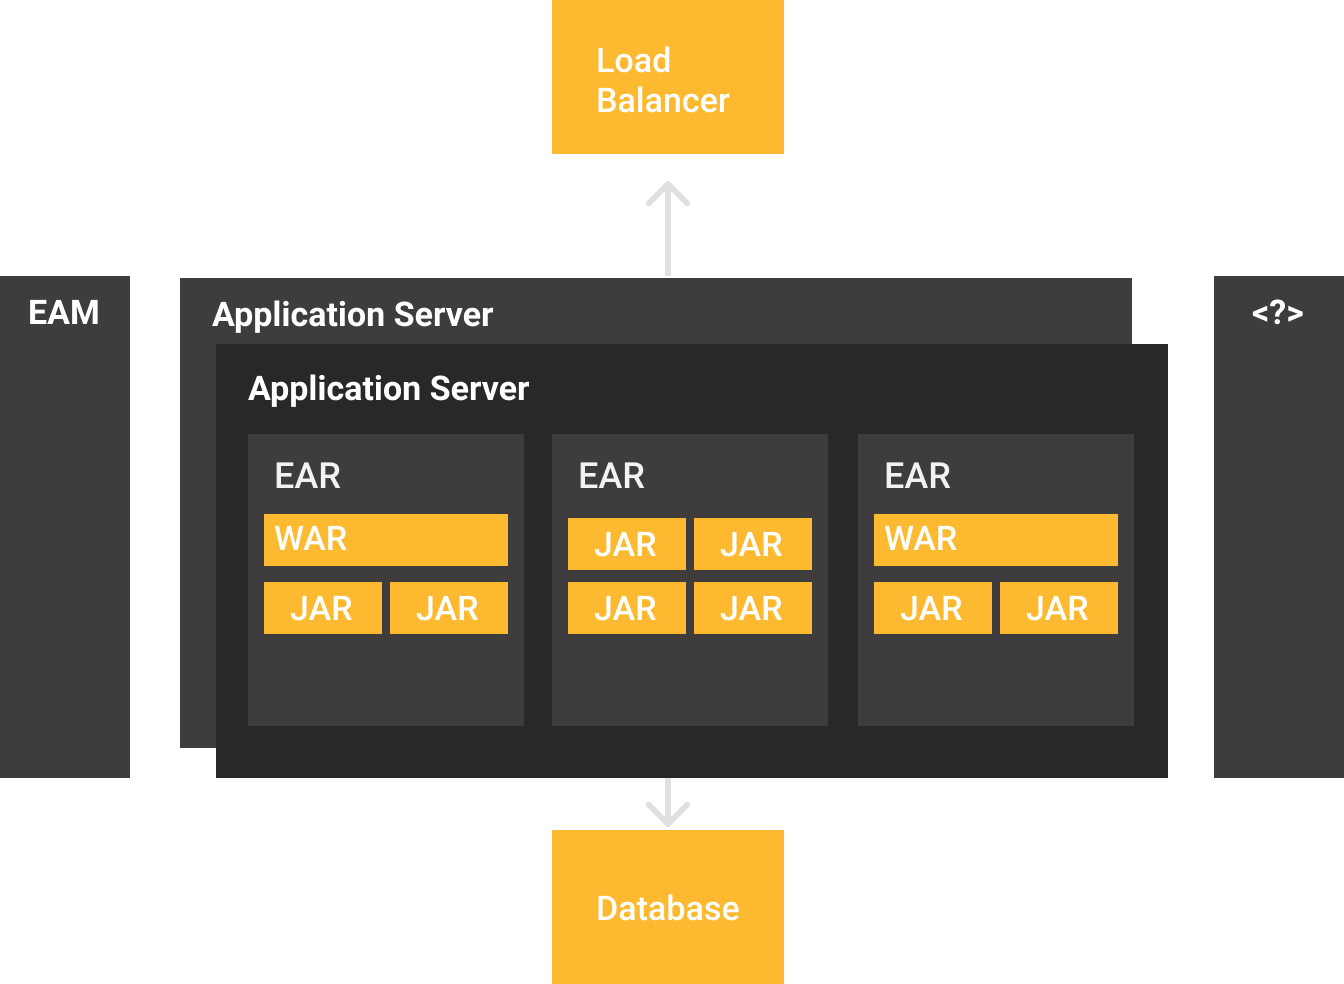
\includegraphics[width=0.6\linewidth]{Images/monolitos}
        \caption{Monólito}
    \end{figure}
\end{frame}

\begin{frame}{ESB}
    \begin{figure}
        \centering
        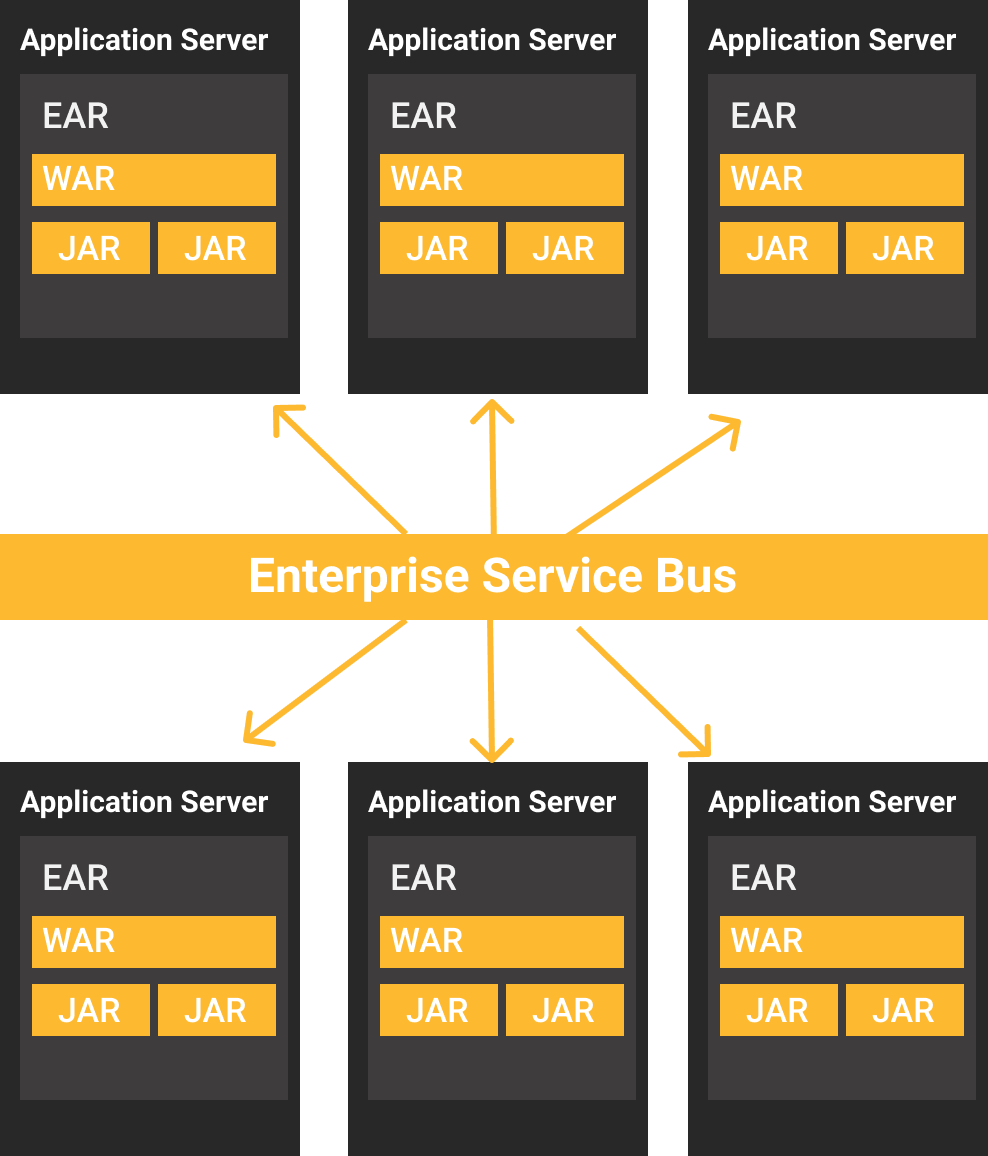
\includegraphics[width=0.4\linewidth]{Images/esb}
        \caption{ESB}
    \end{figure}
\end{frame}



\begin{frame}{Microservicios}
    \begin{figure}
        \centering
        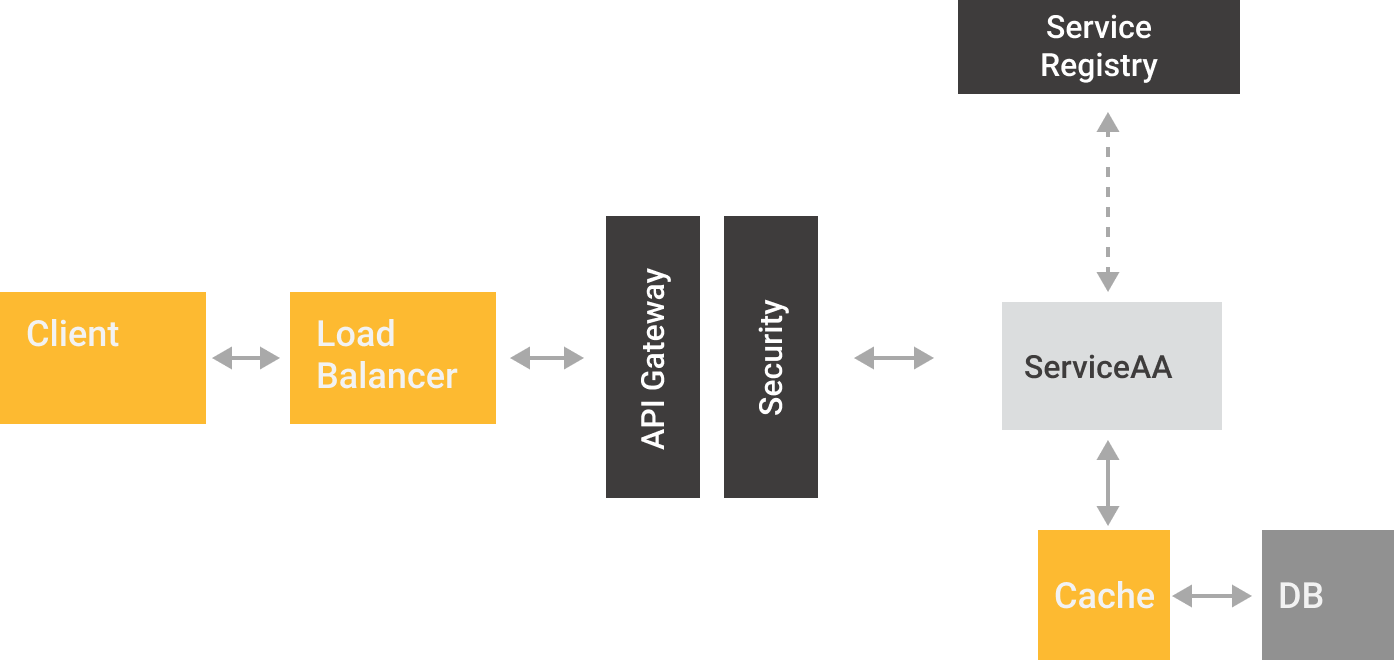
\includegraphics[width=0.7\linewidth]{Images/microservicios}
        \caption{Microservicios}
    \end{figure}
\end{frame}

\begin{frame}{Monolito vs. Microservicios}
    \begin{figure}
        \centering
        
\includegraphics[width=0.6\linewidth]{Images/dukecowboy}
    \end{figure}
\end{frame}


{
    \usebackgroundtemplate{
\includegraphics[width=\paperwidth]{Images/separador}}
    \setbeamercolor{normal text}{fg=white}
    \setbeamercolor{frametitle}{fg=red}
    \usebeamercolor[fg]{normal text}
    \section{Introducción a Docker}
}


\begin{frame}{VMs}
    \begin{figure}
        \centering
        
\includegraphics[width=0.6\linewidth]{Images/virtualbox}
        \label{fig:vm}
    \end{figure}
\end{frame}


\begin{frame}{Hipervisores}
    \begin{figure}
        \centering
        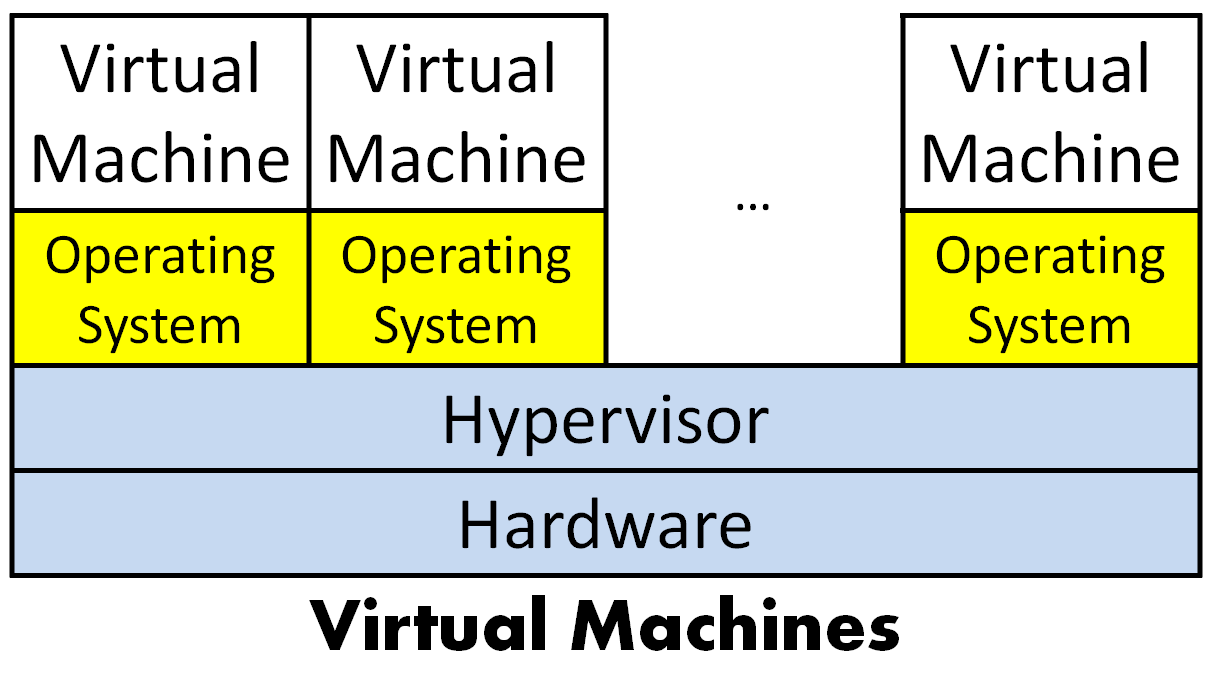
\includegraphics[width=0.6\linewidth]{Images/hypervisors}
        \label{fig:hypervisors}
    \end{figure}
\end{frame}

\begin{frame}{Despliegue contenedores}
    \begin{figure}
        \centering
        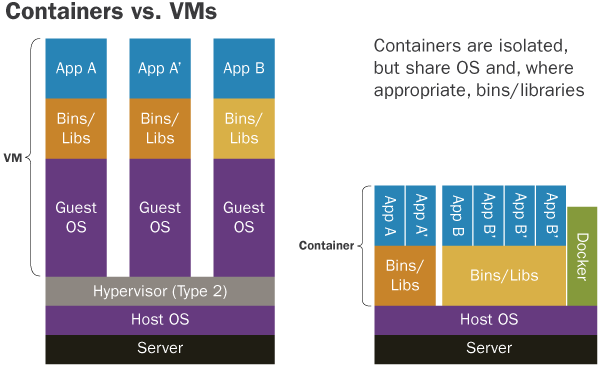
\includegraphics[width=0.7\linewidth]{Images/containervsvm.png}
        \label{fig:containervsvm}
    \end{figure}
\end{frame}

\begin{frame}{Contenedor}
    Contenedor = bibliotecas + app + shell
    \begin{figure}
        \centering
        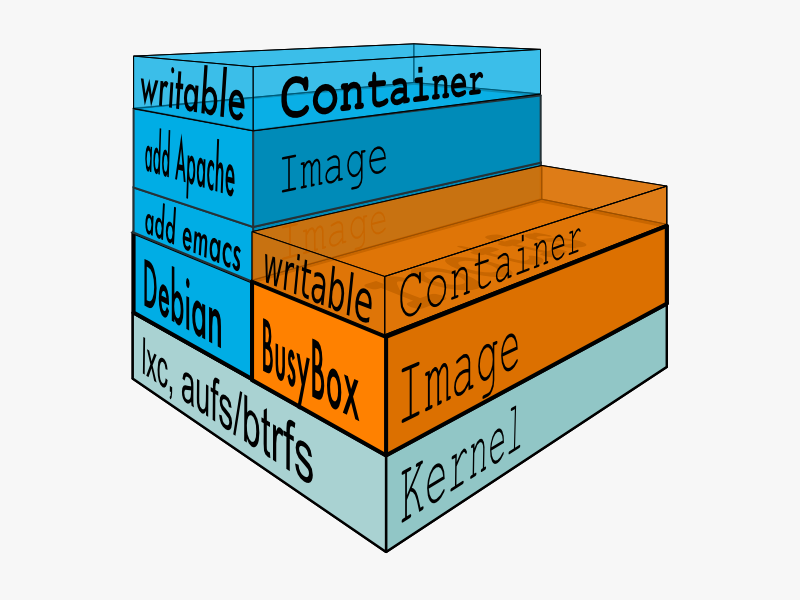
\includegraphics[width=0.6\linewidth]{Images/container.png}
        \label{fig:container}
    \end{figure}
\end{frame}

\begin{frame}{Contenedor}
    Contenedor = bibliotecas + app + shell\\
    
    Ideas generales:
    \begin{itemize}
        \item Distribución
        \item Volatilidad
        \item Automatización
    \end{itemize}
\end{frame}


\begin{frame}{Docker}
    \begin{itemize}
        \item Cgroups + Namespace: Isolamiento de recursos de un grupo y visibilidad entre procesos
        \item libcontainer (LXC/Libvirt/systemd-nspawn)
        \item SELinux, AppArmor, Netfilter
        \item Ventajas: Boot time, menos overhead
        \item Desventajas: Deprecated en Kubernetes, Linux
    \end{itemize}
\end{frame}


\begin{frame}{Demo 1}
    \begin{itemize}
        \item Imagen base (ubuntu)
        \item Ejecución
        \item Agregar paquete
        \item Commit
        \item Ejecución
    \end{itemize}
\end{frame}

\begin{frame}[fragile]{Demo 1}
\begin{lstlisting}
docker pull ubuntu
docker run ubuntu echo "Hola ubuntu"
docker run -it ubuntu /bin/bash
apt-get update && apt-get install nginx
docker ps
docker commit -id- tuxtor/nginx
docker run -d -p 81:80 tuxtor/nginx
\end{lstlisting}
\end{frame}


	\section{Aplicaciones Java}



\begin{frame}{Aplicaciones Java}
    \begin{figure}
        \centering
        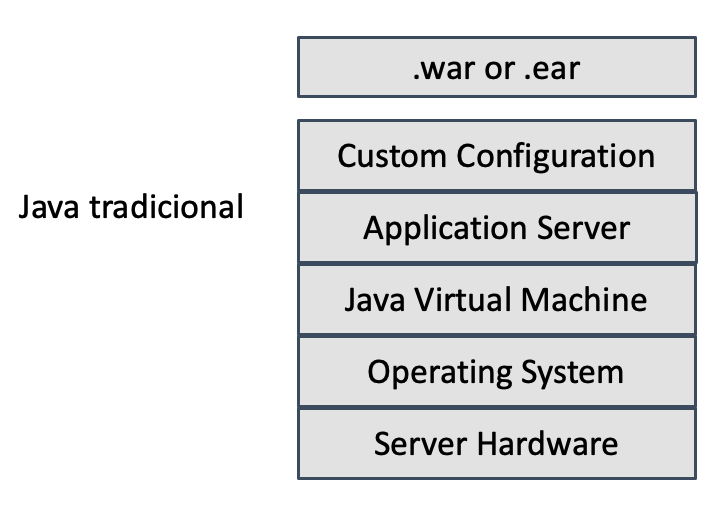
\includegraphics[width=0.5\linewidth]{Images/javatradicional}
    \end{figure}
\end{frame}

\begin{frame}{Aplicaciones Java}
	Formas de despliegue
    \begin{itemize}
        \item War sobre un contenedor o app server
        \item Microservicio como UberJar o FatJar
        \item Microservicio en Docker
    \end{itemize}
\end{frame} 

\begin{frame}{War sobre app server}
Características
    \begin{itemize}
        \item Todos los app servers tienen imágenes listas
        \item Configuración debe ser externalizada
        \item Archivos descriptores (en imagen)
        \item Archivos de configuración de dominio (en imagen)
        \item Archivos properties (en war)
    \end{itemize}
\end{frame} 


\begin{frame}{Demo 1}
App Server completo
\end{frame}


\begin{frame}{Microservicio como UberJar/FatJar}
    \begin{itemize}
        \item El jar no requiere entorno para ejecutarse, solo JVM
        \item Configuración debe ser externalizada
        \item Archivos de configuración de dominio (en imagen)
        \item \textbf{Archivos descriptores} (en war)
        \item \textbf{Configuración mediante archivos properties} (en war)
    \end{itemize}
\end{frame} 


\begin{frame}{Demo 2}
Microservicio como FatJar + Docker + Config + Payara Micro
\end{frame}

\begin{frame}{Microservicio en Docker}
    \begin{itemize}
        \item ThinJar
        \item ThinJar - Mi código
        \item Container - Dependencias/runtime
        \item Archivos de configuración de dominio (en imagen)
        \item \textbf{Archivos descriptores} (en war)
        \item \textbf{Configuración mediante archivos properties} (en war)
    \end{itemize}
\end{frame} 

\begin{frame}{Demo 3}
    Microservicio como ThinJar + Docker + Payara Micro
\end{frame}


\begin{frame}{Límites de memoria}
    \begin{figure}
        \centering
        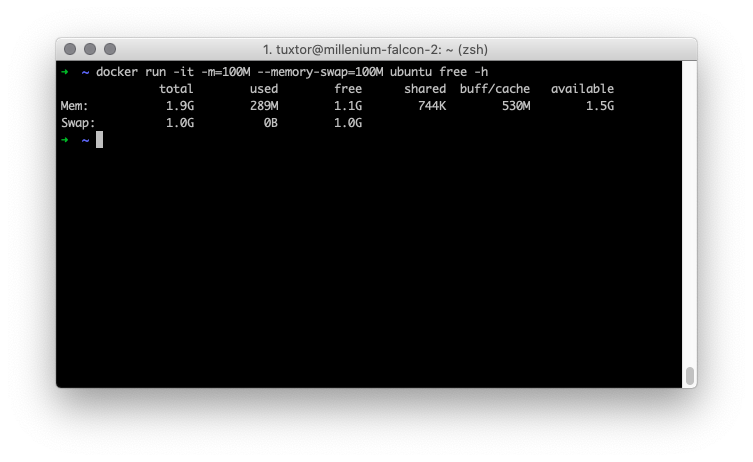
\includegraphics[width=0.9\linewidth]{Images/dockermem.png}
        \label{fig:container1}
    \end{figure}
\end{frame}

\begin{frame}{Límites de memoria - JVM}
    \begin{figure}
        \centering
        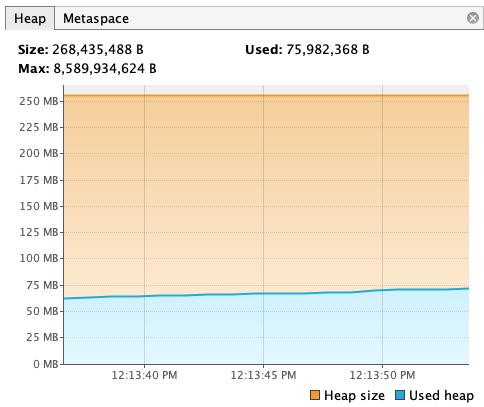
\includegraphics[width=0.6\linewidth]{Images/jvmnolimit.png}
        \label{fig:container2}
    \end{figure}
\end{frame}

\begin{frame}{Límites de memoria - JVM}
    \begin{figure}
        \centering
        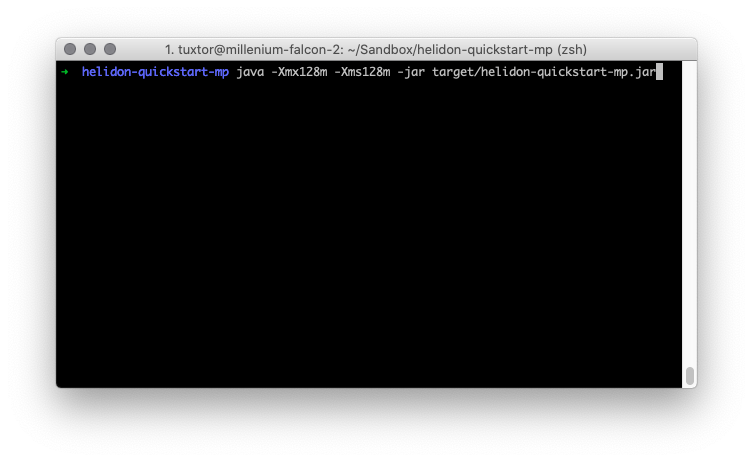
\includegraphics[width=0.9\linewidth]{Images/helidonmem.png}
        \label{fig:container3}
    \end{figure}
\end{frame}

\begin{frame}{Límites de memoria - JVM}
    \begin{figure}
        \centering
        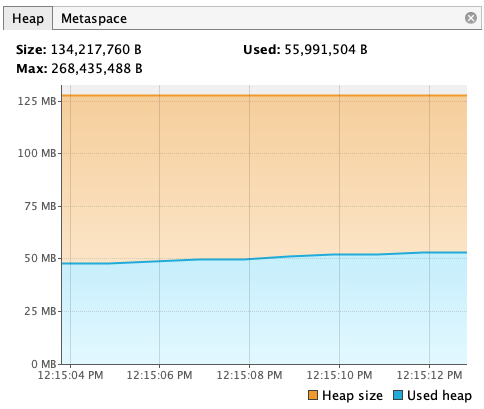
\includegraphics[width=0.6\linewidth]{Images/jvmlimit.png}
        \label{fig:container4}
    \end{figure}
\end{frame}

\begin{frame}{Límites de memoria}
    \begin{figure}
        \centering
        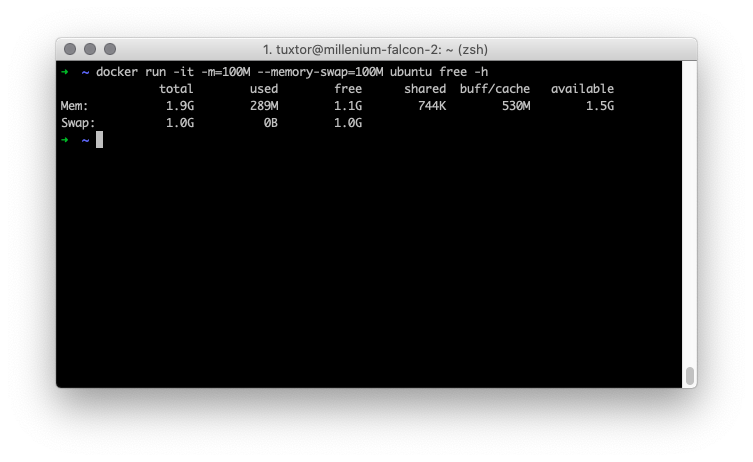
\includegraphics[width=0.9\linewidth]{Images/dockermem.png}
        \label{fig:container5}
    \end{figure}
\end{frame}

\begin{frame}[fragile]{Java Options}
    \begin{lstlisting}
    CMD java -XX:+PrintFlagsFinal -XX:+PrintGCDetails $JAVA_OPTIONS -jar java-container.jar
    \end{lstlisting}
\end{frame}

{
    \usebackgroundtemplate{
\includegraphics[width=\paperwidth]{Images/separador}}
    \setbeamercolor{normal text}{fg=white}
    \setbeamercolor{frametitle}{fg=red}
    \usebeamercolor[fg]{normal text}
    \section{APIs vs Service Mesh}
}

\begin{frame}{APIs}
    \begin{figure}
        \centering
        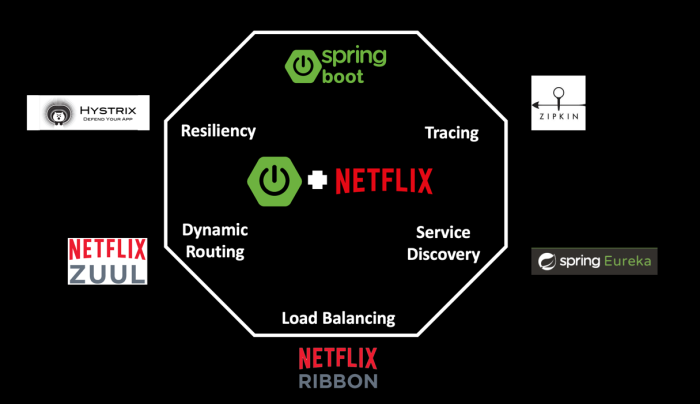
\includegraphics[width=0.7\linewidth]{Images/netflix.png}
        \label{fig:containe6r}
    \end{figure}
\end{frame}

\begin{frame}{APIs}
    \begin{figure}
        \centering
        
\includegraphics[width=0.7\linewidth]{Images/microprofile.png}
        \label{fig:containe7r}
    \end{figure}
\end{frame}


\begin{frame}{APIs}
    \begin{itemize}
        \item REST API
        \item Configuration
        \item Discovery
        \item REST Client
        \item Monitoring
        \item Authentication
        \item Logging
        \item Resilience
    \end{itemize}
\end{frame}

\begin{frame}{APIs - Spring}
    \begin{itemize}
        \item REST API - Spring Rest
        \item Configuration - Spring Config
        \item Discovery - Eureka, Zuul
        \item REST Client - Spring RestTemkplate
        \item Monitoring y tracing - Zipkin
        \item Authentication - Spring security
        \item Logging - Kibana
        \item Resilience - Hystrix
    \end{itemize}
\end{frame}

\begin{frame}{APIs - Basadas en Java/Jakarta EE}
    \begin{itemize}
        \item REST API - JAX-RS
        \item Configuration - MicroProfile Config
        \item Discovery - Ad-hoc/Zookeeper
        \item REST Client - MicroProfile Client
        \item Monitoring y tracing - MicroProfile Healthcheck
        \item Authentication - MicroProfile JWT
        \item Logging - Kibana 
        \item Resilience - MicroProfile Fault Tolerance
    \end{itemize}
\end{frame}

\begin{frame}{El camino a Kubernetes}
    \begin{figure}
        \centering
        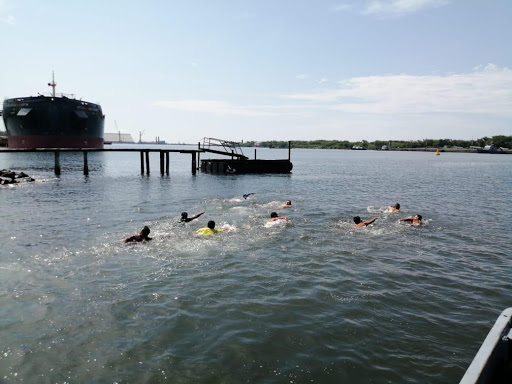
\includegraphics[width=0.5\linewidth]{Images/run}
    \end{figure}
\end{frame}


\begin{frame}{El camino a Kubernetes}
    \begin{figure}
        \centering
        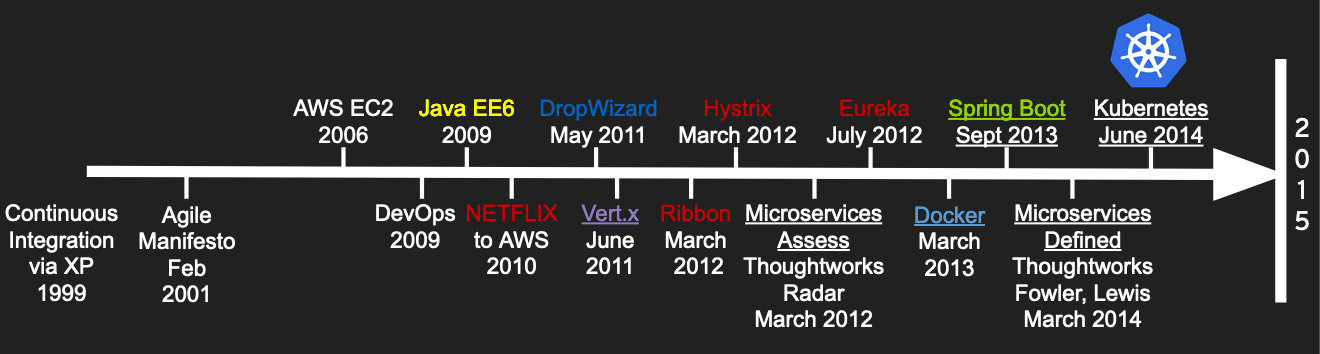
\includegraphics[width=\linewidth]{Images/timeline.png}
        \label{fig:contai8ner}
    \end{figure}

    Créditos: Rafael Benevides
\end{frame}



\begin{frame}{Kubernetes}
    \begin{figure}
        \centering
        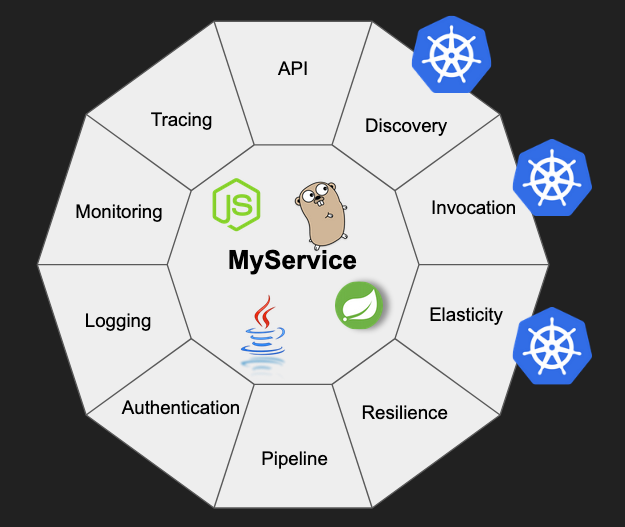
\includegraphics[width=0.5\linewidth]{Images/kube1.png}
        \label{fig:contain9er}
    \end{figure}
    
    Créditos: Rafael Benevides
\end{frame}


\begin{frame}{Kubernetes}
    \begin{figure}
        \centering
        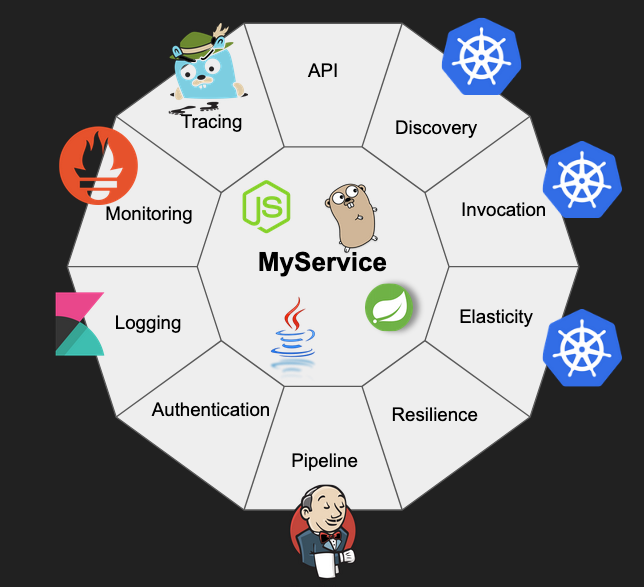
\includegraphics[width=0.5\linewidth]{Images/kube2.png}
        \label{fig:contain10er}
    \end{figure}
    
    Créditos: Rafael Benevides
\end{frame}


\begin{frame}{Kubernetes}
    \begin{figure}
        \centering
        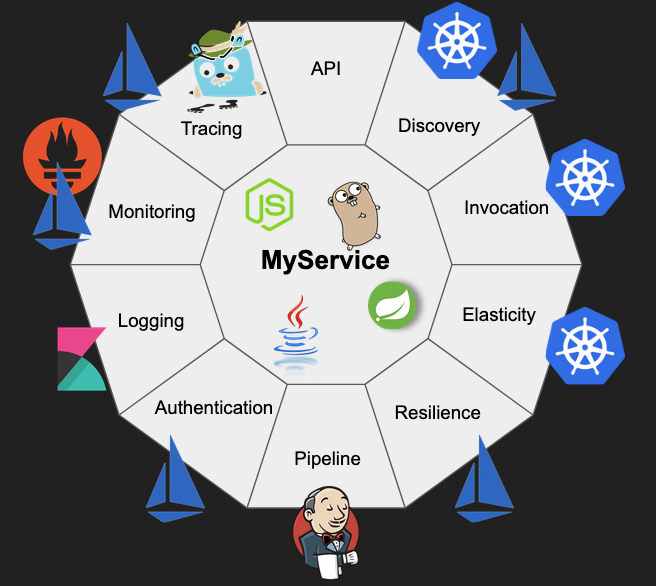
\includegraphics[width=0.5\linewidth]{Images/kube3.png}
        \label{fig:containe11r}
    \end{figure}
    
    Créditos: Rafael Benevides
\end{frame}

\begin{frame}{Kubernetes}
    \begin{figure}
        \centering
        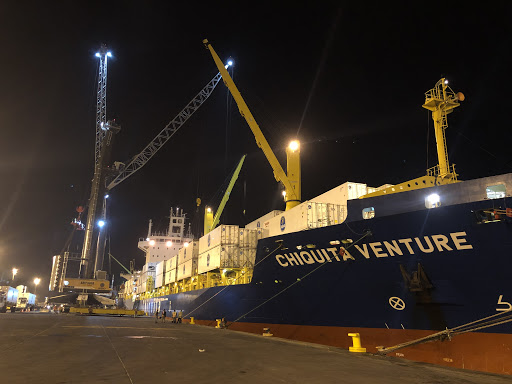
\includegraphics[width=0.8\linewidth]{Images/kubquetzal}
    \end{figure}
\end{frame}



\begin{frame}{Kubernetes - Pod}

            \begin{alertblock}{¿Que es un pod?}
                \begin{itemize}
                    \item Uno o más contenedores
                    \item IP Compartida
                    \item Caen todos o ninguno (ciclo de vida)
                    \item Storage compartido
                    \item Recursos compartidos
                \end{itemize}
            \end{alertblock}

\end{frame}

\begin{frame}{Kubernetes - Deployment}

    \begin{alertblock}{¿Que es un deployment?}
        Descriptor que mantiene el número de PODs replicas en ejecución. Describe un estado
    \end{alertblock}

    
\end{frame}


\begin{frame}{Kubernetes - Servicios}
    
    \begin{alertblock}{¿Que es un servicio?}
        Agrupación de PODs, -e.g. una IP estable virtual y un nombre de DNS si se requiere-
    \end{alertblock}
    
    
\end{frame}

\begin{frame}{Víctor Orozco}
\begin{columns}[T] % contents are top vertically aligned
	
	\begin{column}[T]{4cm} % alternative top-align that's better for graphics
		\begin{figure}
			\centering
			
\includegraphics[width=\linewidth]{Images/logos}
		\end{figure}
	\end{column}
	\begin{column}[T]{6cm} % each column can also be its own environment
		\begin{itemize}
			\item vorozco@nabenik.com
			\item \href{https://twitter.com/tuxtor}{@tuxtor}
			\item \href{http://vorozco.com}{http://vorozco.com}
			\item \href{http://tuxtor.shekalug.org}{http://tuxtor.shekalug.org} 
		\end{itemize}
		\begin{center}
			
\includegraphics[width=0.1\linewidth]{Images/cclogo}
			\\
			This work is licensed under Creative Commons Attribution-NonCommercial-ShareAlike 3.0 Guatemala (CC BY-NC-SA 3.0 GT).
		\end{center}
	\end{column}
\end{columns}
\end{frame}

{
    \usebackgroundtemplate{
\includegraphics[width=\paperwidth]{Images/final}}
    \begin{frame}
    \end{frame}
}


\end{document}

